% GR to QFT Connection Diagram
% File: tikz_gr_to_qft.tex
% Purpose: Visualize mathematical path from general relativity to quantum field theory
% For: Chapter 1 - Mathematical Preliminaries

\begin{figure}[htbp]
\centering
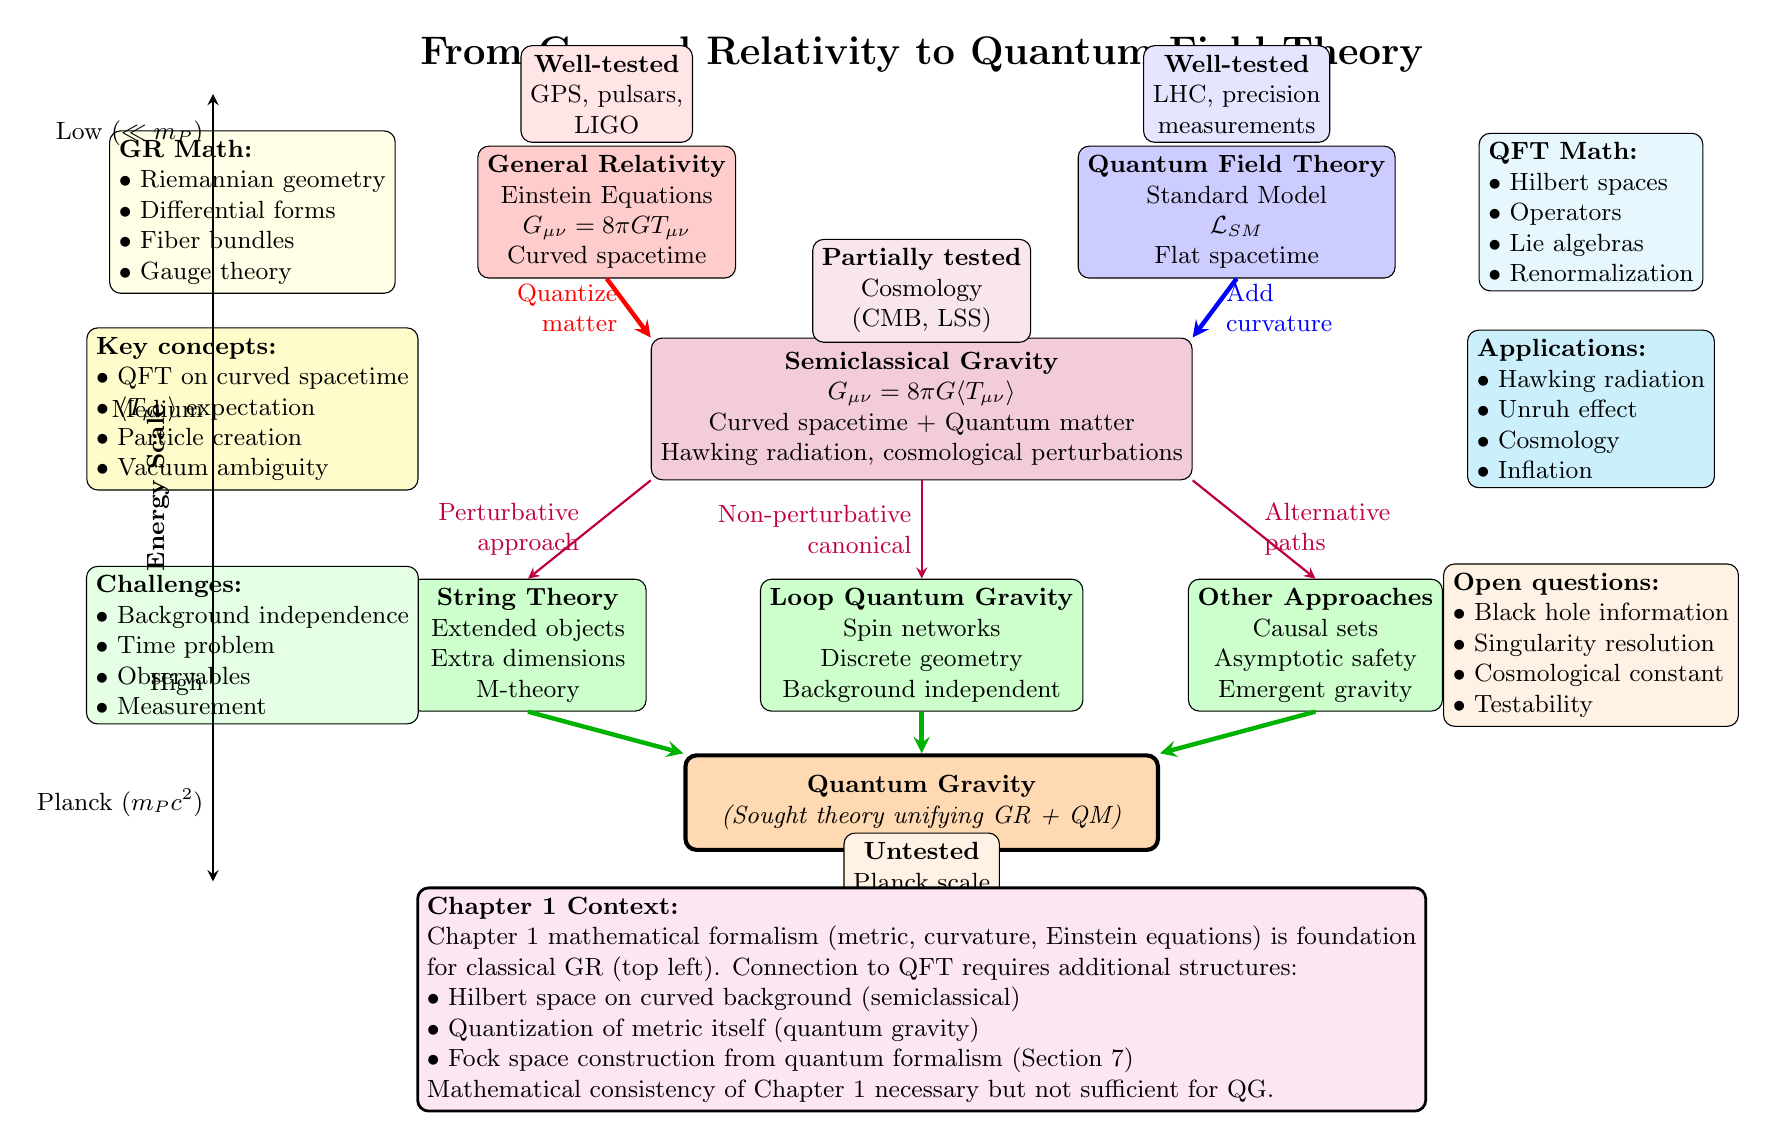
\begin{tikzpicture}[scale=1.0, every node/.style={font=\small}]

% Title
\node[font=\bfseries\Large] at (7, 9) {From General Relativity to Quantum Field Theory};

% Top: Classical GR
\node[draw, fill=red!20, rounded corners, align=center, minimum width=3cm, minimum height=1.5cm] (gr) at (3, 7) {
    \textbf{General Relativity}\\
    Einstein Equations\\
    $G_{\mu\nu} = 8\pi G T_{\mu\nu}$\\
    Curved spacetime
};

% Classical QFT (separate)
\node[draw, fill=blue!20, rounded corners, align=center, minimum width=3cm, minimum height=1.5cm] (qft) at (11, 7) {
    \textbf{Quantum Field Theory}\\
    Standard Model\\
    $\mathcal{L}_{\text{SM}}$\\
    Flat spacetime
};

% Middle level: Semiclassical
\node[draw, fill=purple!20, rounded corners, align=center, minimum width=6cm, minimum height=1.8cm] (semiclassical) at (7, 4.5) {
    \textbf{Semiclassical Gravity}\\
    $G_{\mu\nu} = 8\pi G \langle T_{\mu\nu} \rangle$\\
    Curved spacetime + Quantum matter\\
    Hawking radiation, cosmological perturbations
};

% Lower level: Approaches to quantum gravity
\node[draw, fill=green!20, rounded corners, align=center, minimum width=3cm, minimum height=1.5cm] (strings) at (2, 1.5) {
    \textbf{String Theory}\\
    Extended objects\\
    Extra dimensions\\
    M-theory
};

\node[draw, fill=green!20, rounded corners, align=center, minimum width=3cm, minimum height=1.5cm] (lqg) at (7, 1.5) {
    \textbf{Loop Quantum Gravity}\\
    Spin networks\\
    Discrete geometry\\
    Background independent
};

\node[draw, fill=green!20, rounded corners, align=center, minimum width=3cm, minimum height=1.5cm] (other) at (12, 1.5) {
    \textbf{Other Approaches}\\
    Causal sets\\
    Asymptotic safety\\
    Emergent gravity
};

% Bottom: Unified theory
\node[draw, fill=orange!30, rounded corners, align=center, minimum width=6cm, minimum height=1.2cm, line width=1.5pt] (qg) at (7, -0.5) {
    \textbf{Quantum Gravity}\\
    \emph{(Sought theory unifying GR + QM)}
};

% Arrows: Classical to semiclassical
\draw[->, >=stealth, ultra thick, red] (gr.south) -- (semiclassical.north west) node[midway, left, align=right] {Quantize\\matter};
\draw[->, >=stealth, ultra thick, blue] (qft.south) -- (semiclassical.north east) node[midway, right, align=left] {Add\\curvature};

% Arrows: Semiclassical to approaches
\draw[->, >=stealth, thick, purple] (semiclassical.south west) -- (strings.north) node[midway, left, align=right] {Perturbative\\approach};
\draw[->, >=stealth, thick, purple] (semiclassical.south) -- (lqg.north) node[midway, left, align=right] {Non-perturbative\\canonical};
\draw[->, >=stealth, thick, purple] (semiclassical.south east) -- (other.north) node[midway, right, align=left] {Alternative\\paths};

% Arrows: Approaches to quantum gravity
\draw[->, >=stealth, ultra thick, green!70!black] (strings.south) -- (qg.north west);
\draw[->, >=stealth, ultra thick, green!70!black] (lqg.south) -- (qg.north);
\draw[->, >=stealth, ultra thick, green!70!black] (other.south) -- (qg.north east);

% Key mathematical structures (side annotations)
\node[draw, fill=yellow!10, align=left, rounded corners] at (-1.5, 7) {
    \textbf{GR Math:}\\
    $\bullet$ Riemannian geometry\\
    $\bullet$ Differential forms\\
    $\bullet$ Fiber bundles\\
    $\bullet$ Gauge theory
};

\node[draw, fill=cyan!10, align=left, rounded corners] at (15.5, 7) {
    \textbf{QFT Math:}\\
    $\bullet$ Hilbert spaces\\
    $\bullet$ Operators\\
    $\bullet$ Lie algebras\\
    $\bullet$ Renormalization
};

\node[draw, fill=yellow!20, align=left, rounded corners] at (-1.5, 4.5) {
    \textbf{Key concepts:}\\
    $\bullet$ QFT on curved spacetime\\
    $\bullet$ $\langle T_{\mu\nu} \rangle$ expectation\\
    $\bullet$ Particle creation\\
    $\bullet$ Vacuum ambiguity
};

\node[draw, fill=cyan!20, align=left, rounded corners] at (15.5, 4.5) {
    \textbf{Applications:}\\
    $\bullet$ Hawking radiation\\
    $\bullet$ Unruh effect\\
    $\bullet$ Cosmology\\
    $\bullet$ Inflation
};

\node[draw, fill=green!10, align=left, rounded corners] at (-1.5, 1.5) {
    \textbf{Challenges:}\\
    $\bullet$ Background independence\\
    $\bullet$ Time problem\\
    $\bullet$ Observables\\
    $\bullet$ Measurement
};

\node[draw, fill=orange!10, align=left, rounded corners] at (15.5, 1.5) {
    \textbf{Open questions:}\\
    $\bullet$ Black hole information\\
    $\bullet$ Singularity resolution\\
    $\bullet$ Cosmological constant\\
    $\bullet$ Testability
};

% Energy scales
\draw[<->, >=stealth, thick] (-2, -1.5) -- (-2, 8.5);
\node[rotate=90] at (-2.7, 3.5) {\textbf{Energy Scale}};

\node[left] at (-2, 8) {Low ($\ll m_P$)};
\node[left] at (-2, 4.5) {Medium};
\node[left] at (-2, 1) {High};
\node[left] at (-2, -0.5) {Planck ($m_P c^2$)};

% Experimental status
\node[draw, fill=red!10, align=center, rounded corners] at (3, 8.5) {
    \textbf{Well-tested}\\
    GPS, pulsars,\\
    LIGO
};

\node[draw, fill=blue!10, align=center, rounded corners] at (11, 8.5) {
    \textbf{Well-tested}\\
    LHC, precision\\
    measurements
};

\node[draw, fill=purple!10, align=center, rounded corners] at (7, 6) {
    \textbf{Partially tested}\\
    Cosmology\\
    (CMB, LSS)
};

\node[draw, fill=orange!10, align=center, rounded corners] at (7, -1.5) {
    \textbf{Untested}\\
    Planck scale\\
    $\sim 10^{19}$ GeV
};

% Chapter 1 context box
\node[draw, fill=magenta!10, align=left, rounded corners, line width=1pt] at (7, -3) {
    \textbf{Chapter 1 Context:}\\
    Chapter 1 mathematical formalism (metric, curvature, Einstein equations) is foundation\\
    for classical GR (top left). Connection to QFT requires additional structures:\\
    $\bullet$ Hilbert space on curved background (semiclassical)\\
    $\bullet$ Quantization of metric itself (quantum gravity)\\
    $\bullet$ Fock space construction from quantum formalism (Section 7)\\
    Mathematical consistency of Chapter 1 necessary but not sufficient for QG.
};

\end{tikzpicture}
\caption{Mathematical and conceptual pathway from classical general relativity (top left) and quantum field theory on flat spacetime (top right) through semiclassical gravity (middle) to sought quantum gravity theory (bottom). Energy scales on left, experimental status indicated. Chapter 1 formalism provides classical GR foundation; additional mathematical structures needed for quantum regime. Multiple approaches to quantum gravity shown (string theory, loop quantum gravity, alternatives) with current status. Key challenges and open questions annotated.}
\label{fig:gr_to_qft}
\end{figure}
